\documentclass[10pt,a4paper]{article}
\usepackage[T1]{fontenc}
\usepackage[utf8]{inputenc}
\usepackage[margin=23mm]{geometry}
\usepackage{amsmath,graphicx,booktabs,float,microtype}
\usepackage[colorlinks=true,urlcolor=blue]{hyperref}
\setlength{\parindent}{0pt}\setlength{\parskip}{4pt}
\newcommand{\code}[1]{\texttt{\detokenize{#1}}}
\newcommand{\OriginalAttentionBA}{0.584}
\newcommand{\ControlledAttentionFoneBA}{0.620}
\newcommand{\ControlledAttentionBABA}{0.629}
\newcommand{\TrackDelta}{0.039}
\newcommand{\TrackLooLow}{0.034}
\newcommand{\TrackLooHigh}{0.044}
\newcommand{\BassFprDrumsOn}{0.503}
\newcommand{\BassFprDrumsOff}{0.276}

\begin{document}
\begin{center}\Large\bfseries ELEC5305 Project: Supplementary Diagnostics\end{center}
\begin{center}Ryan Hu -- SID 550275044 -- Review V4\end{center}
\subsection*{Additional frozen-checkpoint diagnostics}
The following analysis completes the comparison of frame scores, attention and relative weighted contribution on the controlled data. It reuses the already inspected v2 test tracks and is therefore a descriptive follow-up, not a new independent test. No network was retrained and the original v2 architecture-selection decision remains unchanged.

The contribution signal is $a_{tc}p_{tc}$, summed into physical time bins and normalised over retained time for the alignment comparison. It indicates the relative distribution of class evidence, not calibrated activity. Because the scales of these signals differ, the diagnostic F1 table selects a separate threshold for each signal and class on validation data. Its operating points differ from the validation-balanced thresholds in the main results and must not be conflated with them.
\begin{table}[H]\centering\small
\caption{Attention-network signal comparison across three seeds. Separate validation-F1 calibration; retrospective descriptive test analysis.}
\begin{tabular}{lrrrrr}\toprule
Signal & Micro P & Micro R & Micro F1 & Macro F1 & Macro BA \\\midrule
frame & 0.630 & 0.878 & 0.733 & 0.718 & 0.603 \\
attention & 0.587 & 0.931 & 0.720 & 0.714 & 0.542 \\
contribution & 0.607 & 0.875 & 0.715 & 0.710 & 0.577 \\
\bottomrule\end{tabular}\end{table}
\begin{table}[H]\centering\small
\caption{Mean class/seed alignment on positive clips. Lift is averaged per clip, not computed as the ratio of the displayed means. Contribution is time-normalised.}
\begin{tabular}{lrrr}\toprule
Signal / scene & Active mass & Active fraction & Lift \\\midrule
attention / original & 0.928 & 0.906 & 1.055 \\
attention / absence & 0.919 & 0.895 & 1.075 \\
attention / transition & 0.681 & 0.466 & 1.519 \\
contribution / original & 0.925 & 0.906 & 1.039 \\
contribution / absence & 0.912 & 0.895 & 1.034 \\
contribution / transition & 0.712 & 0.466 & 1.597 \\
\bottomrule\end{tabular}\end{table}
\begin{table}[H]\centering\small
\caption{Primary frame precision, recall and F1 at the unchanged validation-balanced operating points of the controlled comparison.}
\begin{tabular}{lrrrrrr}\toprule
Model & Micro P & Micro R & Micro F1 & Macro P & Macro R & Macro F1 \\\midrule
baseline & 0.615 & 0.700 & 0.655 & 0.636 & 0.705 & 0.647 \\
attention & 0.658 & 0.754 & 0.702 & 0.656 & 0.743 & 0.689 \\
max & 0.654 & 0.580 & 0.587 & 0.700 & 0.583 & 0.576 \\
\bottomrule\end{tabular}\end{table}
On the controlled transition scenes, attention and weighted contribution can concentrate more mass on active intervals than uniform weights. A lift greater than one establishes relative alignment under these artificial interventions; it does not imply reliable presence/absence estimation. The diagnostic F1 comparison and the per-scene active fractions are needed to interpret that alignment. Neither the lift nor a single illustrative example proves that the model has isolated each instrument's causal acoustic evidence.

Validation-only sensitivity varies threshold offset by $\pm0.10$ and edge-padded smoothing across one, three and five 0.5 s bins. The table reports these perturbations without adopting a new test operating point. This separates investigation of robustness from test-set optimisation. Event extraction remains contiguous positive bins without gap merging or duration filtering; its grid and matching tolerance are fixed and explicitly reported.
\begin{table}[H]\centering\small
\caption{Validation-only sensitivity, averaged over three seeds. No perturbed setting replaces the frozen calibration of the controlled comparison.}
\begin{tabular}{lrrrrr}\toprule
Model & Window bins & Offset & Micro F1 & Macro F1 & Macro BA \\\midrule
baseline & 1 & -0.10 & 0.752 & 0.748 & 0.628 \\
baseline & 1 & +0.00 & 0.734 & 0.727 & 0.663 \\
baseline & 1 & +0.10 & 0.645 & 0.625 & 0.640 \\
baseline & 3 & +0.00 & 0.747 & 0.740 & 0.670 \\
baseline & 5 & +0.00 & 0.749 & 0.742 & 0.668 \\
attention & 1 & -0.10 & 0.789 & 0.779 & 0.702 \\
attention & 1 & +0.00 & 0.764 & 0.755 & 0.714 \\
attention & 1 & +0.10 & 0.709 & 0.700 & 0.697 \\
attention & 3 & +0.00 & 0.786 & 0.776 & 0.719 \\
attention & 5 & +0.00 & 0.790 & 0.780 & 0.717 \\
max & 1 & -0.10 & 0.728 & 0.723 & 0.612 \\
max & 1 & +0.00 & 0.631 & 0.619 & 0.673 \\
max & 1 & +0.10 & 0.457 & 0.437 & 0.621 \\
max & 3 & +0.00 & 0.642 & 0.627 & 0.676 \\
max & 5 & +0.00 & 0.644 & 0.627 & 0.673 \\
\bottomrule\end{tabular}\end{table}

\subsection*{Audible cases and runnable prototype}
Two original validation excerpts are provided with audio, log-mel views, MIDI activity and predictions. They are selected as the highest and lowest clip F1 among excerpts containing a reference transition; silence-only clips are excluded. They deliberately illustrate a success and a failure and are not used as representative test statistics. The report bundle includes the case-selection record and the presentation plays both sounds.

\begin{figure}[H]\centering
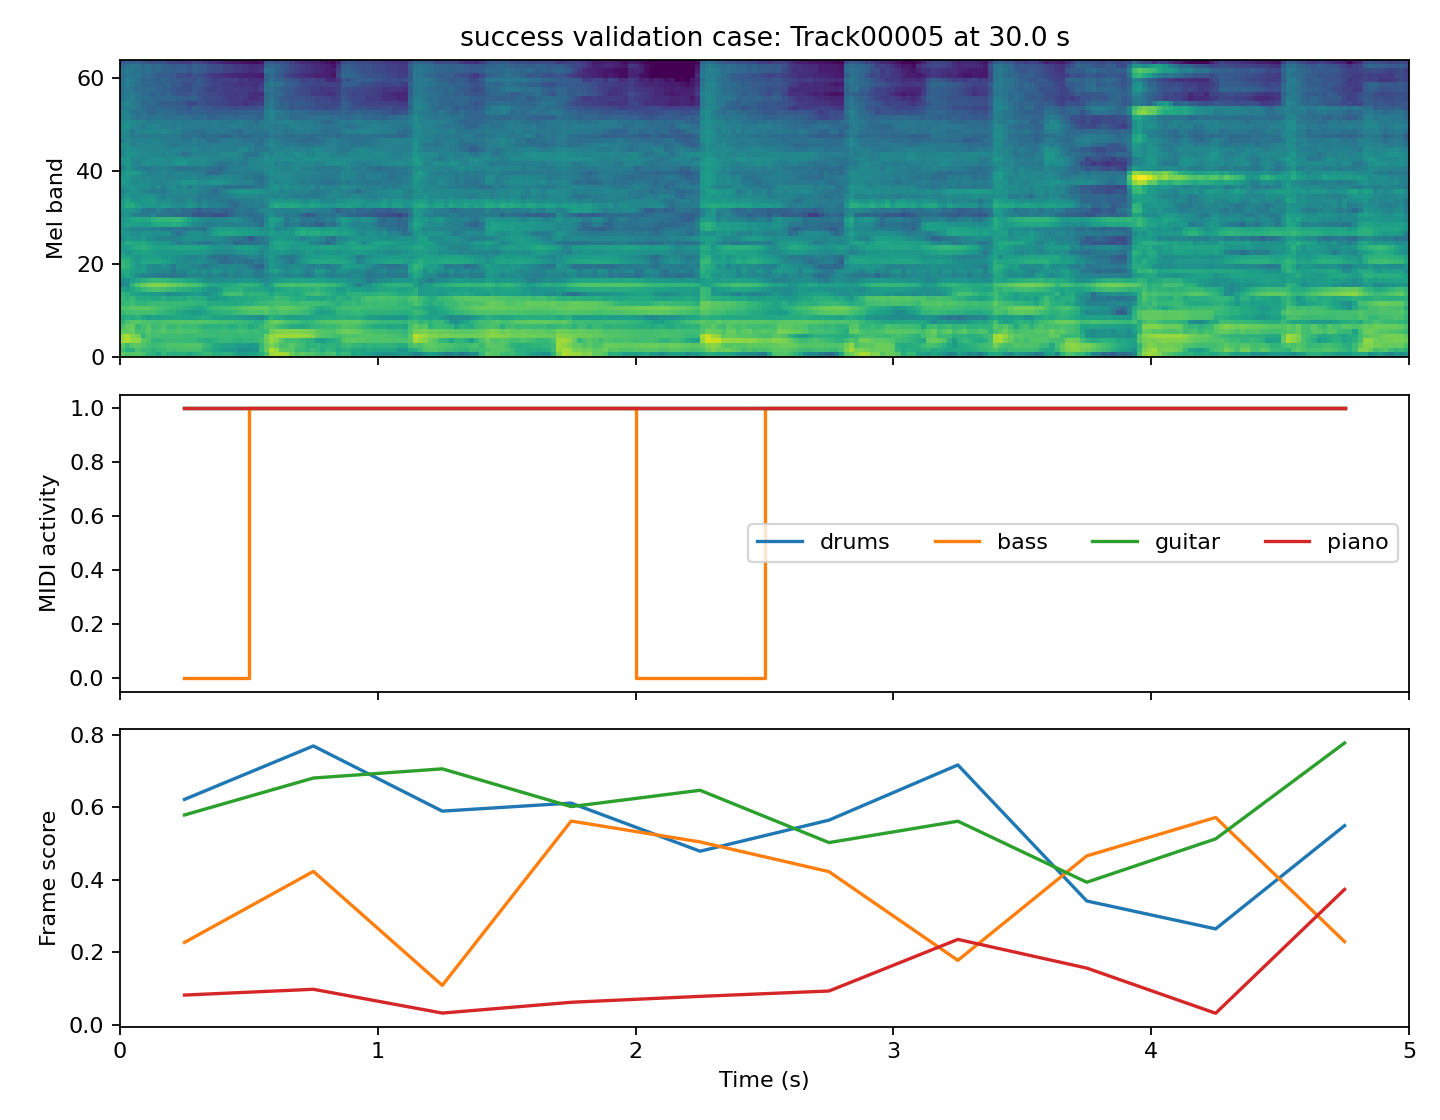
\includegraphics[width=.47\linewidth]{figures/success_validation.png}\hfill
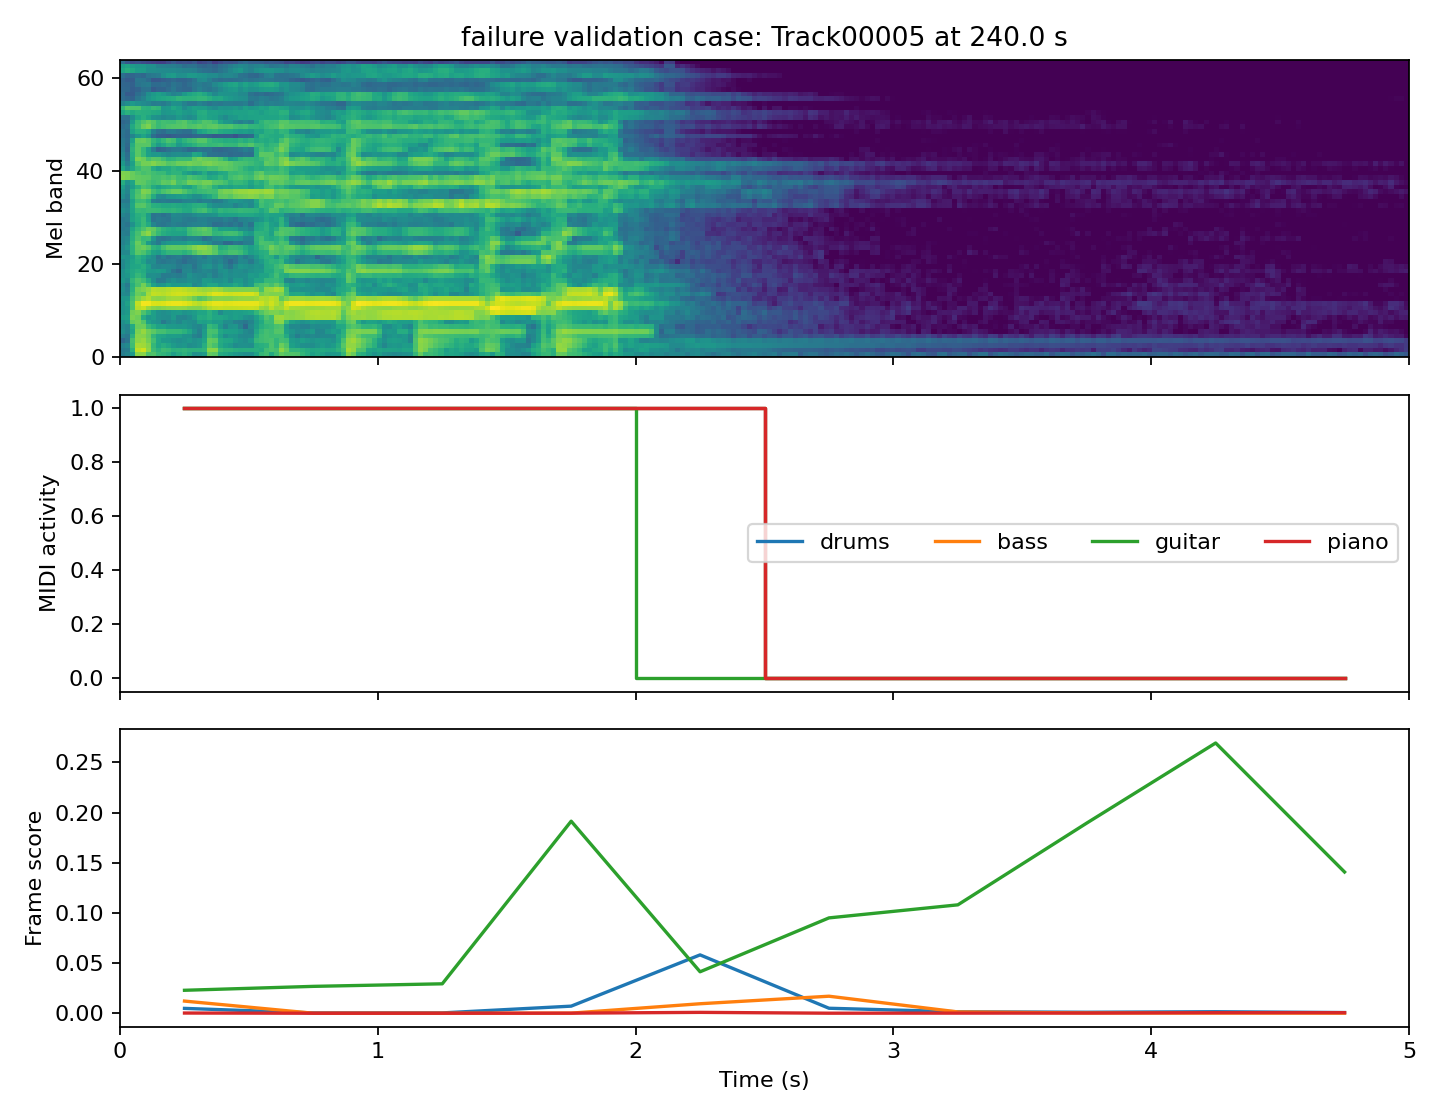
\includegraphics[width=.47\linewidth]{figures/failure_validation.png}
\caption{Deliberately selected validation success and failure. Top: log-mel feature; middle: reference activity; bottom: frame scores. Companion five-second WAV excerpts are supplied for listening. These synthetic excerpts do not establish real-recording performance.}
\end{figure}

The new \code{predict} command loads audio, resamples to the checkpoint rate, applies the same clipped and scaled log-mel transform used in training, and exports a timeline CSV, interval JSON and plot. Its calibration file is bound to the checkpoint SHA-256. Padded final clips are truncated to actual audio duration in the output. This is an executable research prototype; frame scores should not be presented as calibrated probabilities or reliable predictions for arbitrary real music.

\subsection*{Retrospective ablation and error-mechanism checks}
The previous comparison changed both training scenes and clip-checkpoint selection. A completed $2\times2$ analysis now crosses original/controlled training data with F1/balanced-accuracy clip selection, separately for mean and attention pooling. Twelve new runs fill the missing cells; twelve retained runs provide the existing cells. All use seeds 5305--5307, the same encoder and optimiser, timestamp bins, and validation-balanced frame calibration. No test score changes the original architecture winner. This is retrospective development analysis on the same inspected test tracks.
\begin{table}[H]\centering\small
\caption{Retrospective factorial comparison on the controlled test distribution. Means and sample SD over three seeds. All cells use the same validation-balanced frame threshold protocol. The original architecture winner is unchanged.}\label{tab:factorial}
\begin{tabular}{lllrr}\toprule
Model & Training data & Clip selection & Frame BA & Micro F1 \\\midrule
baseline & original & F1 & $0.559 \pm 0.013$ & 0.636 \\
baseline & original & BA & $0.568 \pm 0.006$ & 0.676 \\
baseline & controlled & F1 & $0.589 \pm 0.005$ & 0.655 \\
baseline & controlled & BA & $0.589 \pm 0.005$ & 0.655 \\
attention & original & F1 & $0.570 \pm 0.013$ & 0.643 \\
attention & original & BA & $0.584 \pm 0.007$ & 0.681 \\
attention & controlled & F1 & $0.620 \pm 0.003$ & 0.697 \\
attention & controlled & BA & $0.629 \pm 0.011$ & 0.702 \\
\bottomrule\end{tabular}\end{table}
Under fixed balanced selection, attention's controlled-test frame BA rises from \OriginalAttentionBA{} with original training scenes to \ControlledAttentionBABA{} with controlled training. Under F1 selection, controlled training reaches \ControlledAttentionFoneBA{}. Thus the gain is not explained solely by changing clip selection. The data factor also changes scene count and optimiser exposure: this is evidence for the complete training-data condition, not a pure causal estimate of acoustic augmentation. Paired seed contrasts are in \code{results/ablation_v4/summary.json}.

Attention exceeds mean on all four test tracks. The unweighted controlled-track BA difference is \TrackDelta{}; leaving out any one track gives \TrackLooLow{}--\TrackLooHigh{}. These are descriptive robustness values, not confidence limits or proof of population generalisation.

Among bins with bass absent, mean bass FPR across attention seeds is \BassFprDrumsOn{} when drums are active (1235 reference bins), versus \BassFprDrumsOff{} when drums are absent (1055 bins). Reference bins are correlated and are not independent recordings. Repeating predictions over seeds does not multiply these denominators. Contextual confusion, arrangement, masking and the intervention construction are possible explanations; this association does not prove which acoustic evidence the model causally uses.
\begin{figure}[H]\centering
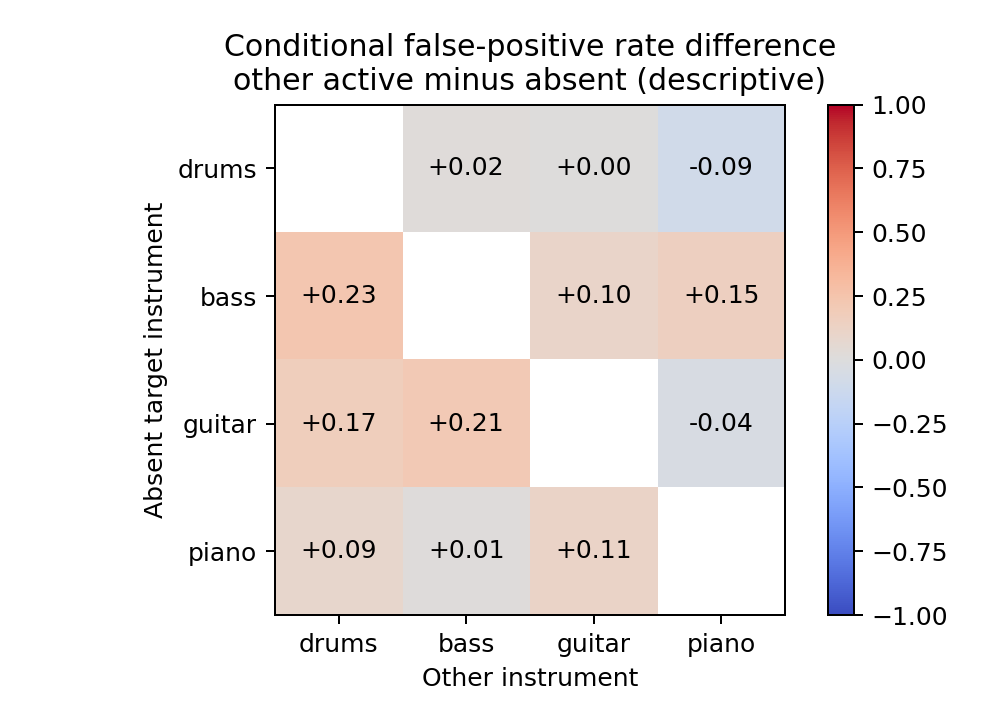
\includegraphics[width=.65\linewidth]{figures/conditional_fpr_v4.png}
\caption{Conditional FPR difference: the target family is absent, while the column family is active versus absent. Mean over three attention seeds; both conditions require at least 20 bins. The diagonal is undefined. These exploratory comparisons share four source tracks.}
\end{figure}

\section*{Reproduction and scope}
All diagnostic CSV files are in \code{results/diagnostics_v3}. The data-root and
checkpoint-root parameters are explicit in \code{scripts/analyse_localisation_signals.py}.
The original v2 runs, model choice and test calibration remain unchanged.
See \code{REPRODUCE.md} for audio inference and the native report build.
\begin{figure}[H]\centering
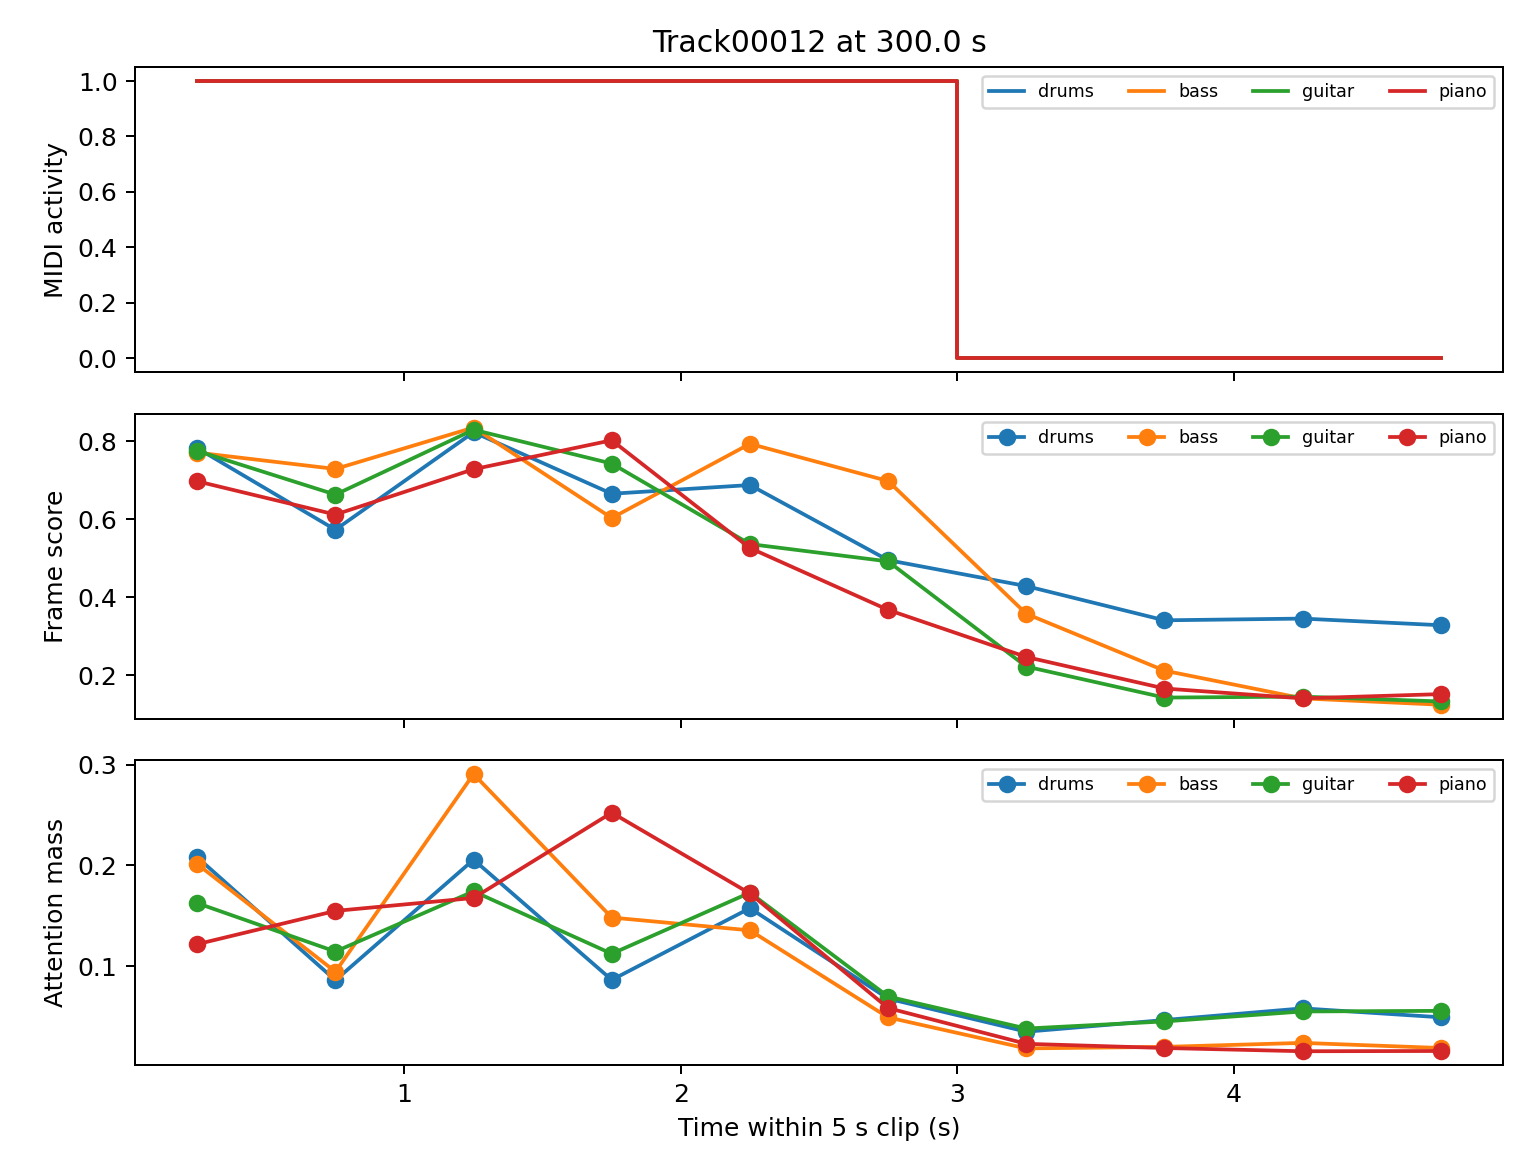
\includegraphics[width=.70\linewidth]{figures/temporal_example.png}
\caption{Historical attention seed 5305 example, Track00012 at 300 s. Selected by reference variation, not model success. Piano becomes inactive near three seconds while other sources remain active; several scores decline together. This does not establish instrument-specific boundary discrimination.}
\end{figure}
\end{document}
